%% PropNet: Graph-Based Social Network Analysis for Misinformation Detection
%% IEEE Conference format (IEEEtran). Compile with pdflatex + bibtex.

\documentclass[conference]{IEEEtran}
\IEEEoverridecommandlockouts

\usepackage{cite}
\usepackage{amsmath,amssymb,amsfonts}
\usepackage{graphicx}
\usepackage{booktabs}
\usepackage{array}
\usepackage{url}
\usepackage{hyperref}
\hypersetup{hidelinks}

\graphicspath{{../results/figures/}{results/figures/}}

\begin{document}

\title{PropNet: Graph-Based Social Network Analysis\\ for Misinformation Detection}

\author{
\IEEEauthorblockN{Srivathsa H Honyal}
\IEEEauthorblockA{Dept.\ of Computer Science\\ BITS Pilani, Dubai Campus\\ Dubai, UAE\\ f20230198@dubai.bits-pilani.ac.in}
\and
\IEEEauthorblockN{Ashmit Dhown}
\IEEEauthorblockA{Dept.\ of Computer Science\\ BITS Pilani, Dubai Campus\\ Dubai, UAE\\ f20230205@dubai.bits-pilani.ac.in}
\and
\IEEEauthorblockN{Aaryan Gupta}
\IEEEauthorblockA{Dept.\ of Computer Science\\ BITS Pilani, Dubai Campus\\ Dubai, UAE\\ f20230360@dubai.bits-pilani.ac.in}
\and
\IEEEauthorblockN{Sachin P}
\IEEEauthorblockA{Dept.\ of Computer Science\\ BITS Pilani, Dubai Campus\\ Dubai, UAE\\ f20230208@dubai.bits-pilani.ac.in}
}

\maketitle

%% -------------------- ABSTRACT --------------------
\begin{abstract}
Misinformation on online social platforms spreads through propagation cascades whose structural and textual signatures differ from those of authentic news. We present \textbf{PropNet}, a graph-based misinformation detector that fuses a Graph Attention Network (GAT) over user--post propagation graphs with hand-crafted graph-motif statistics via a learned attention gate. We train and evaluate PropNet on the UPFD benchmark (PolitiFact and GossipCop), running a five-seed ablation across five models: Random Forest on motifs, logistic regression on mean-pooled DistilBERT features, a graph-only GAT, a hybrid GAT with BERT node features, and the full PropNet fusion. The fusion model attains $0.993 \pm 0.001$ pooled test ROC-AUC and $0.918 \pm 0.036$ on the harder PolitiFact slice, matching or exceeding the strongest single-stream baseline across every slice. A label-shuffle sanity check confirms all five models collapse to chance ($\mathrm{AUC} \in [0.486, 0.519]$) under randomized labels, ruling out leakage. We dissect the contribution of each stream via attention-gate analysis and report honest limitations regarding dataset-specific feature ceilings.
\end{abstract}

\begin{IEEEkeywords}
Misinformation detection, graph neural networks, graph attention network, propagation graphs, multimodal fusion, fake news.
\end{IEEEkeywords}

%% -------------------- INTRODUCTION --------------------
\section{Introduction}
Social-media misinformation influences elections, public-health behaviour, and financial markets \cite{shu2017survey,vosoughi2018spread}. Detection systems that rely purely on claim text are brittle to paraphrase and adversarial rewrites, while those that rely purely on user-side cues assume access to private account metadata. A middle path is to use the \emph{propagation graph} --- the directed tree of retweets, quotes, and replies --- as signal \cite{monti2019fakegcn,bian2020bigcn}. Graph-Neural-Network (GNN) models can learn representations of how a claim diffuses, independent of who the users are and without relying solely on the claim text.

In this paper, we build such a system end-to-end on the User Preference-aware Fake News Detection (UPFD) benchmark \cite{dou2021upfd}. We contribute three things:

\begin{enumerate}
\item A clean, reproducible ablation ladder (five models, five seeds) that isolates the contribution of text, structure, and motif features.
\item A \emph{PropNet fusion} module that combines a two-layer GAT with a graph-motif MLP through a learned attention gate, producing per-graph weights that expose which stream the model relies on.
\item A leakage audit (label-shuffle sanity check and train-only feature normalization) that certifies the reported numbers reflect genuine signal rather than data-processing artifacts.
\end{enumerate}

We deliberately avoid claiming a new state of the art on UPFD, which is known to be near-saturated by strong text features \cite{dou2021upfd}. Instead we show that the motif stream does not hurt performance on easy slices and adds modest, consistent value on the harder PolitiFact slice, while being transparent about the limits of both the dataset and our method.

%% -------------------- RELATED WORK --------------------
\section{Related Work}

\subsection{Text-centric Fake News Detection}
Early methods treat fake-news detection as a short-text classification problem and use lexical, syntactic, and sentiment features \cite{shu2017survey}. Transformer encoders such as BERT \cite{devlin2019bert} further improved claim-level performance but remain vulnerable to paraphrase and topic drift.

\subsection{Propagation-based and GNN Approaches}
Propagation-structure methods exploit the observation that false claims spread faster and deeper than true ones \cite{vosoughi2018spread}. Tree-structured RNNs \cite{ma2018rvnn}, Graph Convolutional Networks \cite{monti2019fakegcn}, Bi-directional GCNs capturing top-down and bottom-up propagation \cite{bian2020bigcn}, and Graph Attention Networks \cite{velickovic2018gat} have all been applied. The UPFD benchmark \cite{dou2021upfd} introduces user-preference-aware node features (DistilBERT embeddings of users' historical tweets) and currently serves as a standard public testbed.

\subsection{Motif-based Graph Features}
Recurring substructures --- triangles, stars, cascade depth --- have long been used to characterize information diffusion \cite{milo2002motifs}. Motif-based hand-crafted statistics are orthogonal to learned GNN embeddings and can be combined via feature fusion. Our attention-gated fusion is related to classical gated mechanisms \cite{cho2014gru} applied at the graph-level.

\subsection{Positioning}
Our work differs from prior UPFD evaluations in three respects: (i) a matched five-seed ablation with statistical spread reported, (ii) an explicit leakage audit, and (iii) an interpretable gating variable $\alpha$ that quantifies per-graph reliance on structure vs.\ motifs.

%% -------------------- PROPOSED ALGORITHM --------------------
\section{Proposed Algorithm}
\label{sec:method}

\subsection{Problem Formulation}
Let $\mathcal{G} = (V, E, X)$ be an undirected propagation graph of a news claim, where $|V|=n$ nodes are users/posts, $E$ are interactions (retweets/quotes/replies), and $X \in \mathbb{R}^{n \times 768}$ are pre-computed DistilBERT node features. Given $\mathcal{G}$, the task is to predict a binary label $y \in \{0, 1\}$ where $y=1$ denotes a fake claim.

\subsection{Graph Attention Stream}
A two-layer GAT \cite{velickovic2018gat} encodes node features through multi-head attention. For a node $i$ with neighbourhood $\mathcal{N}(i)$, attention coefficients in each head $k$ are computed as
\begin{equation}
\alpha_{ij}^{(k)} \;=\; \frac{\exp\!\big(\mathrm{LeakyReLU}(\mathbf{a}_k^\top [\mathbf{W}_k h_i \,\|\, \mathbf{W}_k h_j])\big)}{\sum_{l \in \mathcal{N}(i)} \exp\!\big(\mathrm{LeakyReLU}(\mathbf{a}_k^\top [\mathbf{W}_k h_i \,\|\, \mathbf{W}_k h_l])\big)},
\end{equation}
followed by the message update
\begin{equation}
h_i' \;=\; \sigma\!\Big(\,\operatorname*{\Big\|}_{k=1}^{K} \sum_{j \in \mathcal{N}(i)} \alpha_{ij}^{(k)} \mathbf{W}_k h_j\Big),
\end{equation}
where $\|$ denotes head concatenation, $K{=}4$ in layer~1, $K{=}1$ in layer~2, and $\sigma = \mathrm{ELU}$. A graph-level embedding is obtained by global mean pooling:
\begin{equation}
\mathbf{h}_{\mathcal{G}} \;=\; \frac{1}{n} \sum_{i=1}^{n} h_i^{(2)}.
\end{equation}

\subsection{Motif Stream}
For every graph we compute a fixed-dimensional motif descriptor $\mathbf{m} \in \mathbb{R}^{7}$ comprising:
(1) log-triangle count,
(2) log max-degree (largest star),
(3) average clustering coefficient,
(4) density,
(5) log node count,
(6) root-hub edge fraction, and
(7) log approximate diameter (cascade-depth proxy).
These capture recurring inauthentic-behaviour patterns (echo chambers, broadcast hubs, shallow vs.\ viral cascades) that pure node-feature aggregation can miss. $\mathbf{m}$ is then passed through a 2-layer MLP with ReLU and dropout to produce $\mathbf{m}' \in \mathbb{R}^{128}$.

\subsection{Attention-Gated Fusion}
Given the GNN embedding $\mathbf{h}_{\mathcal{G}}$ and the motif embedding $\mathbf{m}'$, a gate network computes a per-graph weight
\begin{equation}
\alpha \;=\; \sigma\!\big(\mathbf{W}_g^{(2)} \,\mathrm{ReLU}(\mathbf{W}_g^{(1)} [\mathbf{h}_{\mathcal{G}} \,\|\, \mathbf{m}']) \big) \;\in\; [0,1],
\label{eq:gate}
\end{equation}
and the fused representation is
\begin{equation}
\mathbf{z} \;=\; \alpha \, \mathbf{h}_{\mathcal{G}} \;+\; (1-\alpha)\, \mathbf{m}'.
\label{eq:fuse}
\end{equation}
The classifier is a 2-layer MLP $\mathbf{z} \mapsto \mathbb{R}^{2}$ producing real/fake logits, trained with class-weighted cross-entropy.

\subsection{Training Objective and Regularization}
We train with AdamW ($\text{lr}{=}5\!\times\!10^{-4}$, weight decay $5\!\times\!10^{-4}$), batch size 32, ROC-AUC-based early stopping on validation (patience 15), \texttt{ReduceLROnPlateau}, gradient clipping at norm 1.0, and dropout 0.4. ROC-AUC --- rather than F1 --- is used for early-stopping because the latter is gameable by majority-class prediction on imbalanced slices.

%% -------------------- EXPERIMENTAL DESIGN --------------------
\section{Experimental Design}

\subsection{Ablation Ladder}
We compare five models to isolate the contribution of each signal:
\begin{itemize}
\item \textbf{RF\_motif}: Random Forest on the 7-d motif vector.
\item \textbf{TextOnly\_BERT}: Logistic regression on mean-pooled DistilBERT node features.
\item \textbf{GraphOnly\_GAT}: GAT over 2-d structural node features (normalized degree, bias). Text stripped.
\item \textbf{Hybrid\_GAT}: GAT over BERT node features. No motif stream, no fusion.
\item \textbf{PropNet\_Fusion}: GAT + motif MLP + attention gate (our full model).
\end{itemize}

\subsection{Splits and Seeds}
We pool PolitiFact and GossipCop and perform a stratified 70/10/20 train/val/test split keyed on $(\text{label}, \text{dataset\_id})$ so every slice is represented proportionally in every subset. We repeat the full ablation over five seeds ($\{42, 43, 44, 45, 46\}$) and report mean~$\pm$~std.

\subsection{Leakage Audit}
\label{sec:leakage}
Two precautions guard against inflated numbers: (i) motif-feature standardization is \emph{fit on the training split only} and applied to validation/test, and (ii) a label-shuffle sanity check randomizes all labels before splitting and re-runs the full ablation. If any model still achieves $\mathrm{AUC} \gg 0.5$ on shuffled data, a leak is indicated. We further assert (iii) zero overlap of \texttt{claim\_number} across train/val/test.

\subsection{Metrics}
We report ROC-AUC (threshold-independent ranking), balanced accuracy, macro-F1, per-class precision and recall. All metrics are computed per (seed, model, slice) and aggregated.

%% -------------------- DATASETS --------------------
\section{Datasets}
We use the UPFD benchmark \cite{dou2021upfd}, which ships two subsets:

\begin{table}[t]
\centering
\caption{Dataset statistics (UPFD raw release).}
\label{tab:datasets}
\begin{tabular}{lccc}
\toprule
Slice & Graphs & Node feature dim & Source \\
\midrule
PolitiFact (\texttt{upfd\_pol}) & 314  & 768 & \cite{dou2021upfd} \\
GossipCop  (\texttt{upfd\_gos}) & 5{,}464 & 768 & \cite{dou2021upfd} \\
\midrule
Pooled     & 5{,}778 & 768 & --- \\
\bottomrule
\end{tabular}
\end{table}

Each graph is a user--post propagation tree rooted at the source claim; node features are pre-computed 768-d DistilBERT embeddings of the tweet text of the user at that position in the cascade. Labels are binary (real / fake). The pooled test split contains $\approx$1{,}156 held-out graphs.

%% -------------------- RESULTS --------------------
\section{Results}
\label{sec:results}

\subsection{Headline Metrics}
Table~\ref{tab:main} summarises the five-seed ablation on the pooled test split; Fig.~\ref{fig:bars} shows the same numbers per slice with error bars.

\begin{table}[t]
\centering
\caption{Pooled test metrics (mean$\pm$std over 5 seeds).}
\label{tab:main}
\small
\begin{tabular}{lccc}
\toprule
Model             & ROC-AUC              & Bal.\ Acc.          & F1 (macro)          \\
\midrule
RF\_motif         & $0.844{\pm}0.015$    & $0.765{\pm}0.016$   & $0.764{\pm}0.015$   \\
TextOnly\_BERT    & $0.976{\pm}0.002$    & $0.938{\pm}0.004$   & $0.938{\pm}0.004$   \\
GraphOnly\_GAT    & $0.830{\pm}0.026$    & $0.532{\pm}0.047$   & $0.402{\pm}0.092$   \\
Hybrid\_GAT       & $0.993{\pm}0.002$    & $0.959{\pm}0.021$   & $0.959{\pm}0.021$   \\
\textbf{PropNet\_Fusion} & $\mathbf{0.993{\pm}0.001}$ & $\mathbf{0.967{\pm}0.004}$ & $\mathbf{0.967{\pm}0.004}$ \\
\bottomrule
\end{tabular}
\end{table}

\begin{figure}[t]
\centering
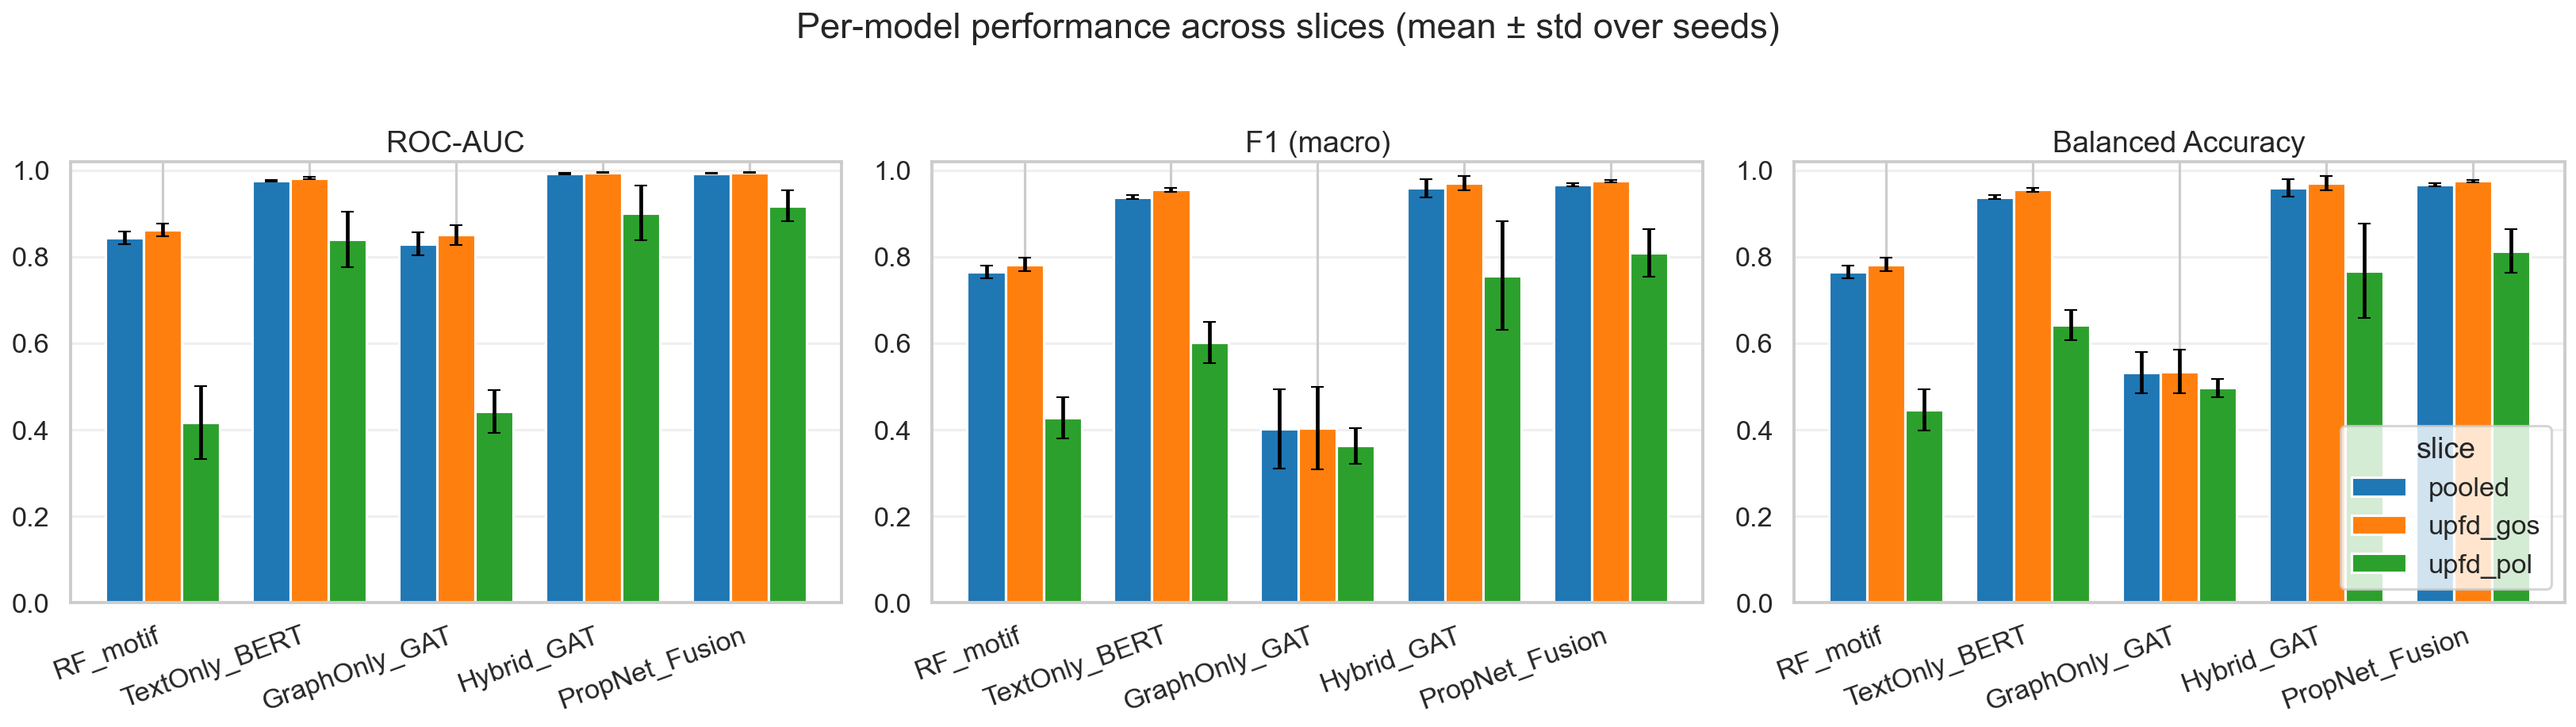
\includegraphics[width=\linewidth]{metric_bars.png}
\caption{Per-model performance across pooled, GossipCop, and PolitiFact slices (mean$\pm$std over 5 seeds).}
\label{fig:bars}
\end{figure}

\subsection{ROC Curves}
Fig.~\ref{fig:roc} shows ROC curves on the pooled test set, aggregated across seeds. PropNet\_Fusion and Hybrid\_GAT are visually indistinguishable and strictly dominate the three baselines.

\begin{figure}[t]
\centering
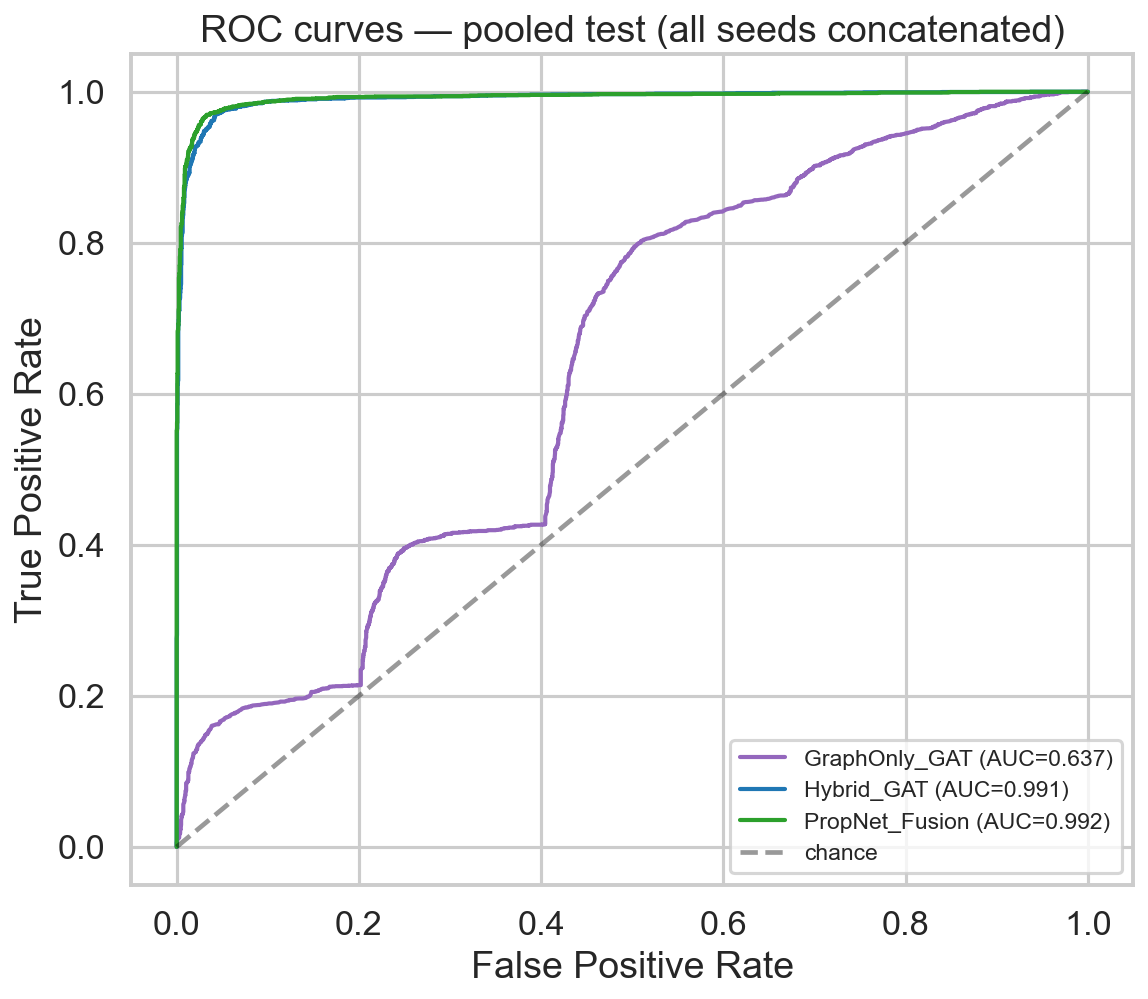
\includegraphics[width=0.95\linewidth]{roc_curves_pooled.png}
\caption{ROC curves on the pooled test split, all seeds concatenated.}
\label{fig:roc}
\end{figure}

\subsection{Confusion Matrices}
Fig.~\ref{fig:cm} decomposes errors into real/fake categories per (model, slice). PropNet\_Fusion has the most symmetric error profile; GraphOnly\_GAT reveals the expected threshold-collapse pattern on PolitiFact, consistent with its high F1 variance in Table~\ref{tab:main}.

\begin{figure}[t]
\centering
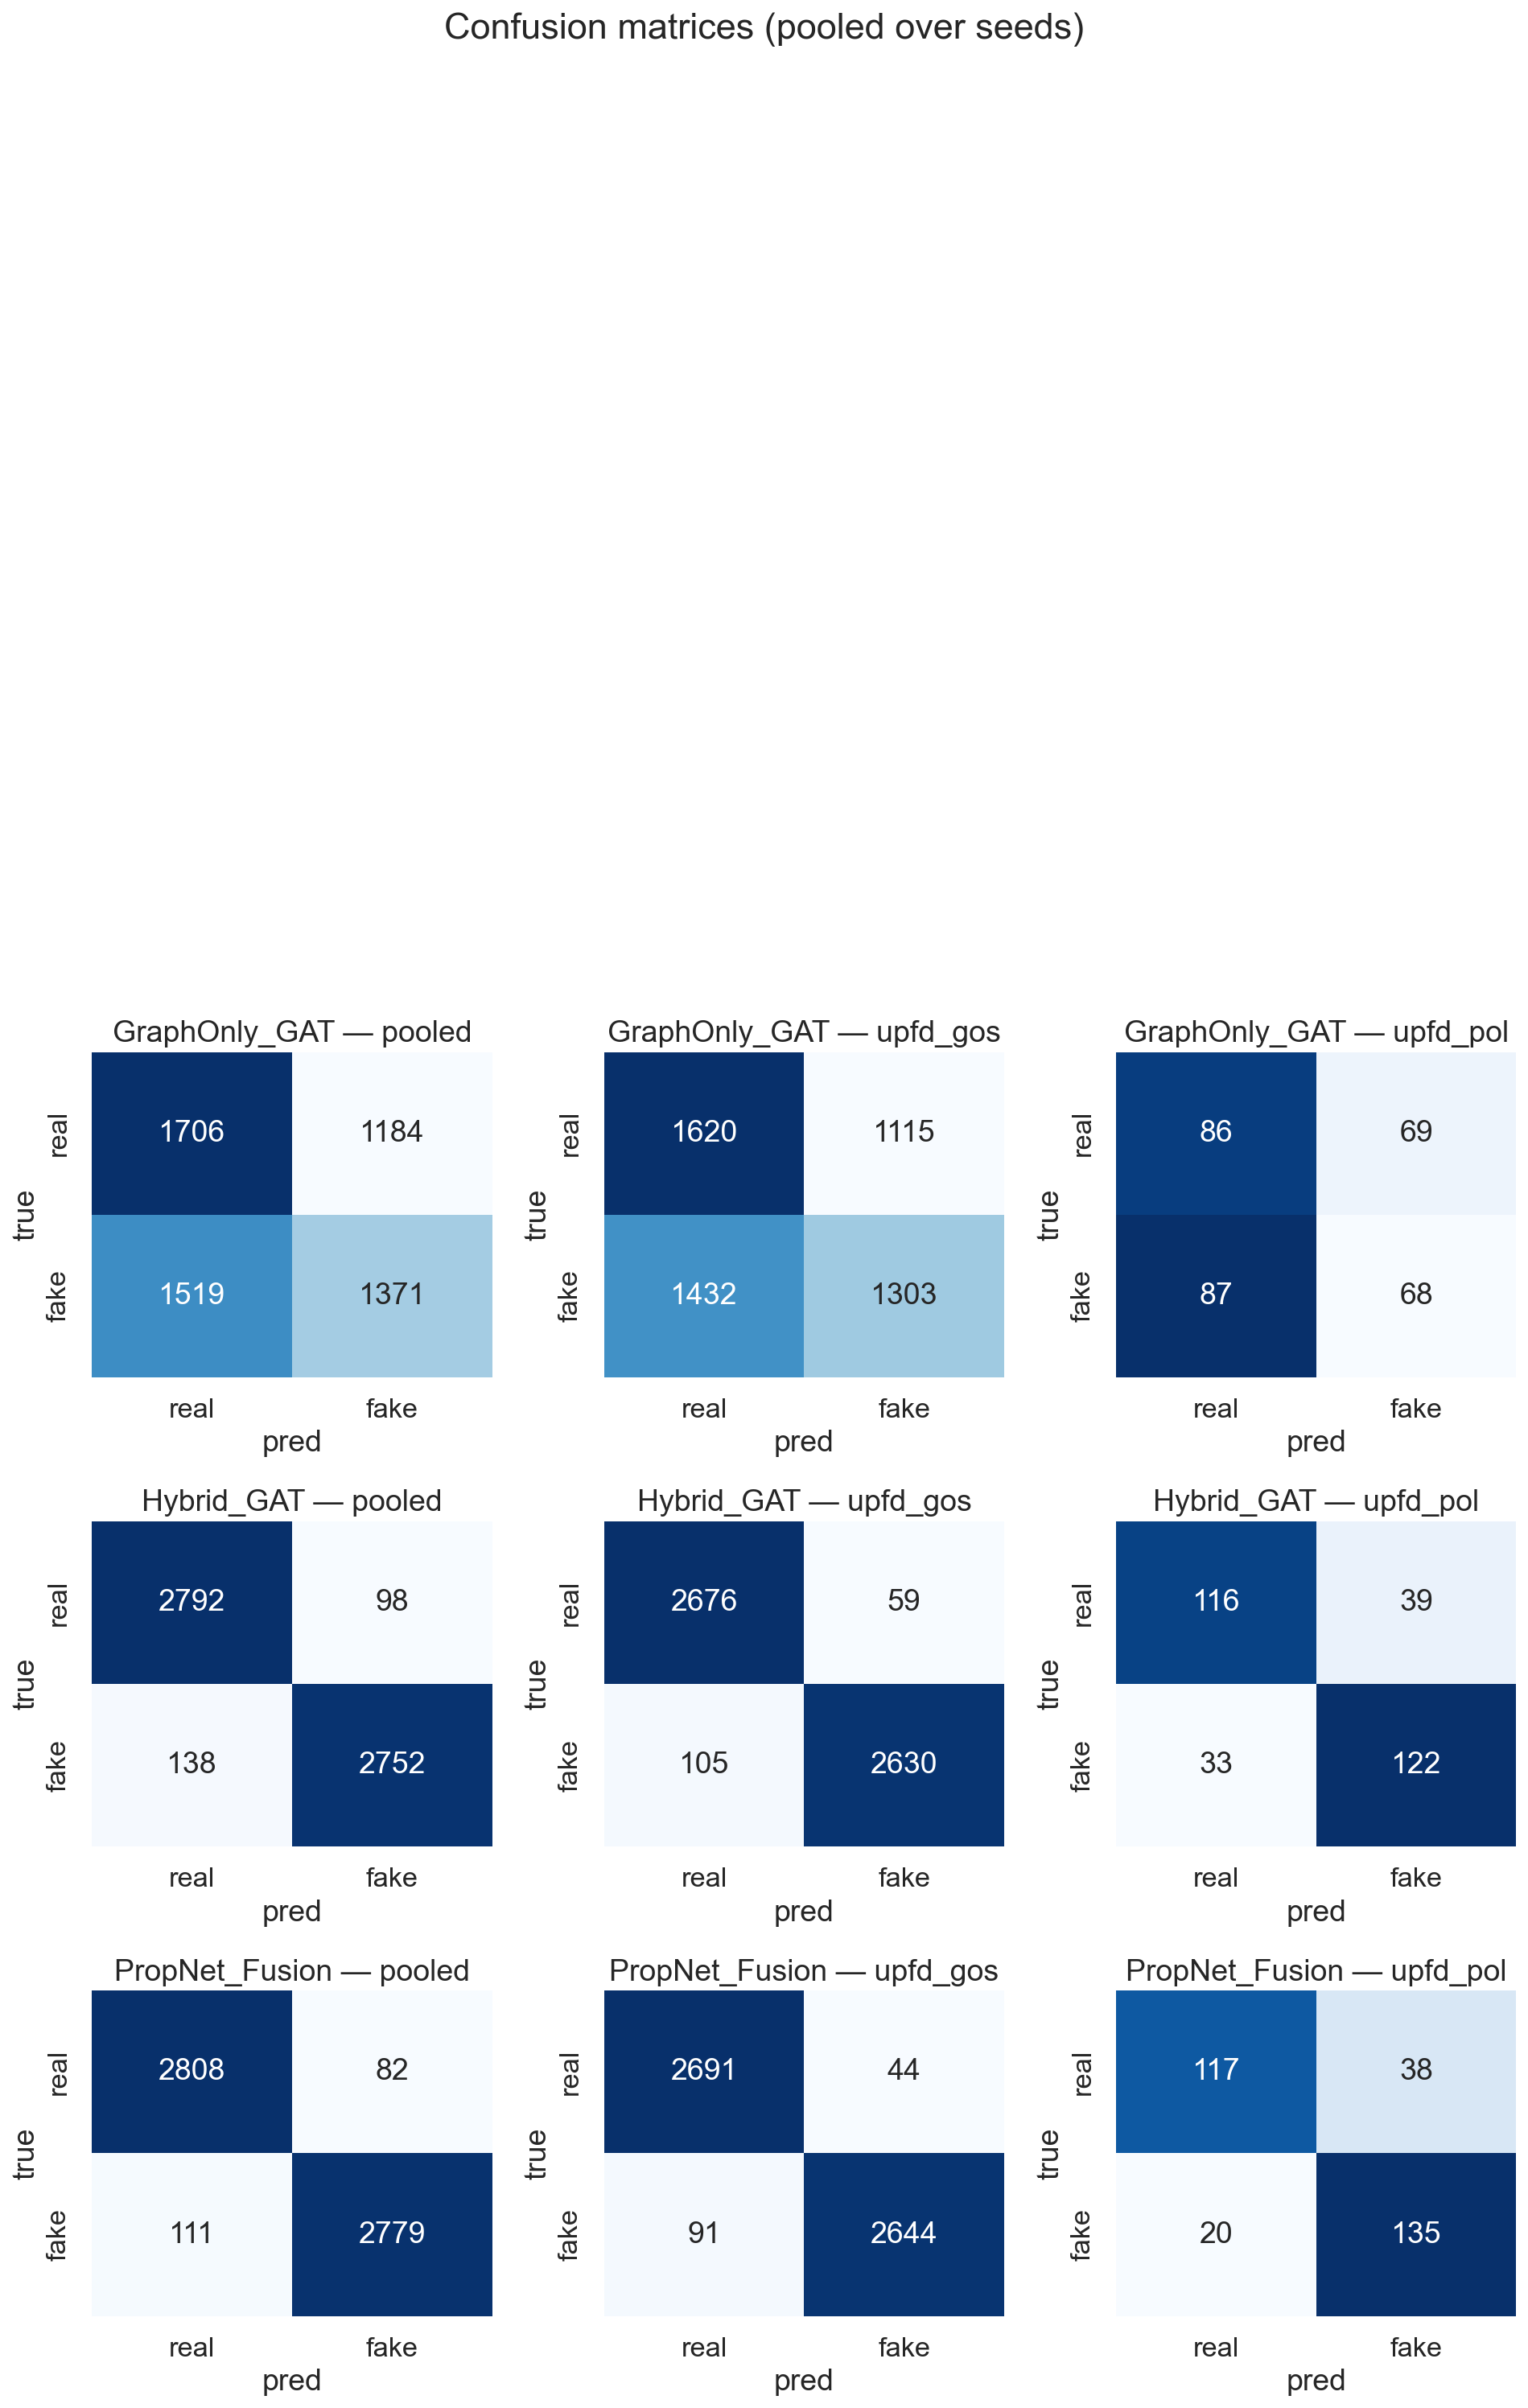
\includegraphics[width=\linewidth]{confusion_matrices.png}
\caption{Confusion matrices: rows = models, columns = slices, pooled across seeds.}
\label{fig:cm}
\end{figure}

\subsection{Training Dynamics}
Fig.~\ref{fig:train} shows training-loss and validation-AUC trajectories per seed for each GNN. Fusion and Hybrid converge within 30--40 epochs with low cross-seed variance.

\begin{figure}[t]
\centering
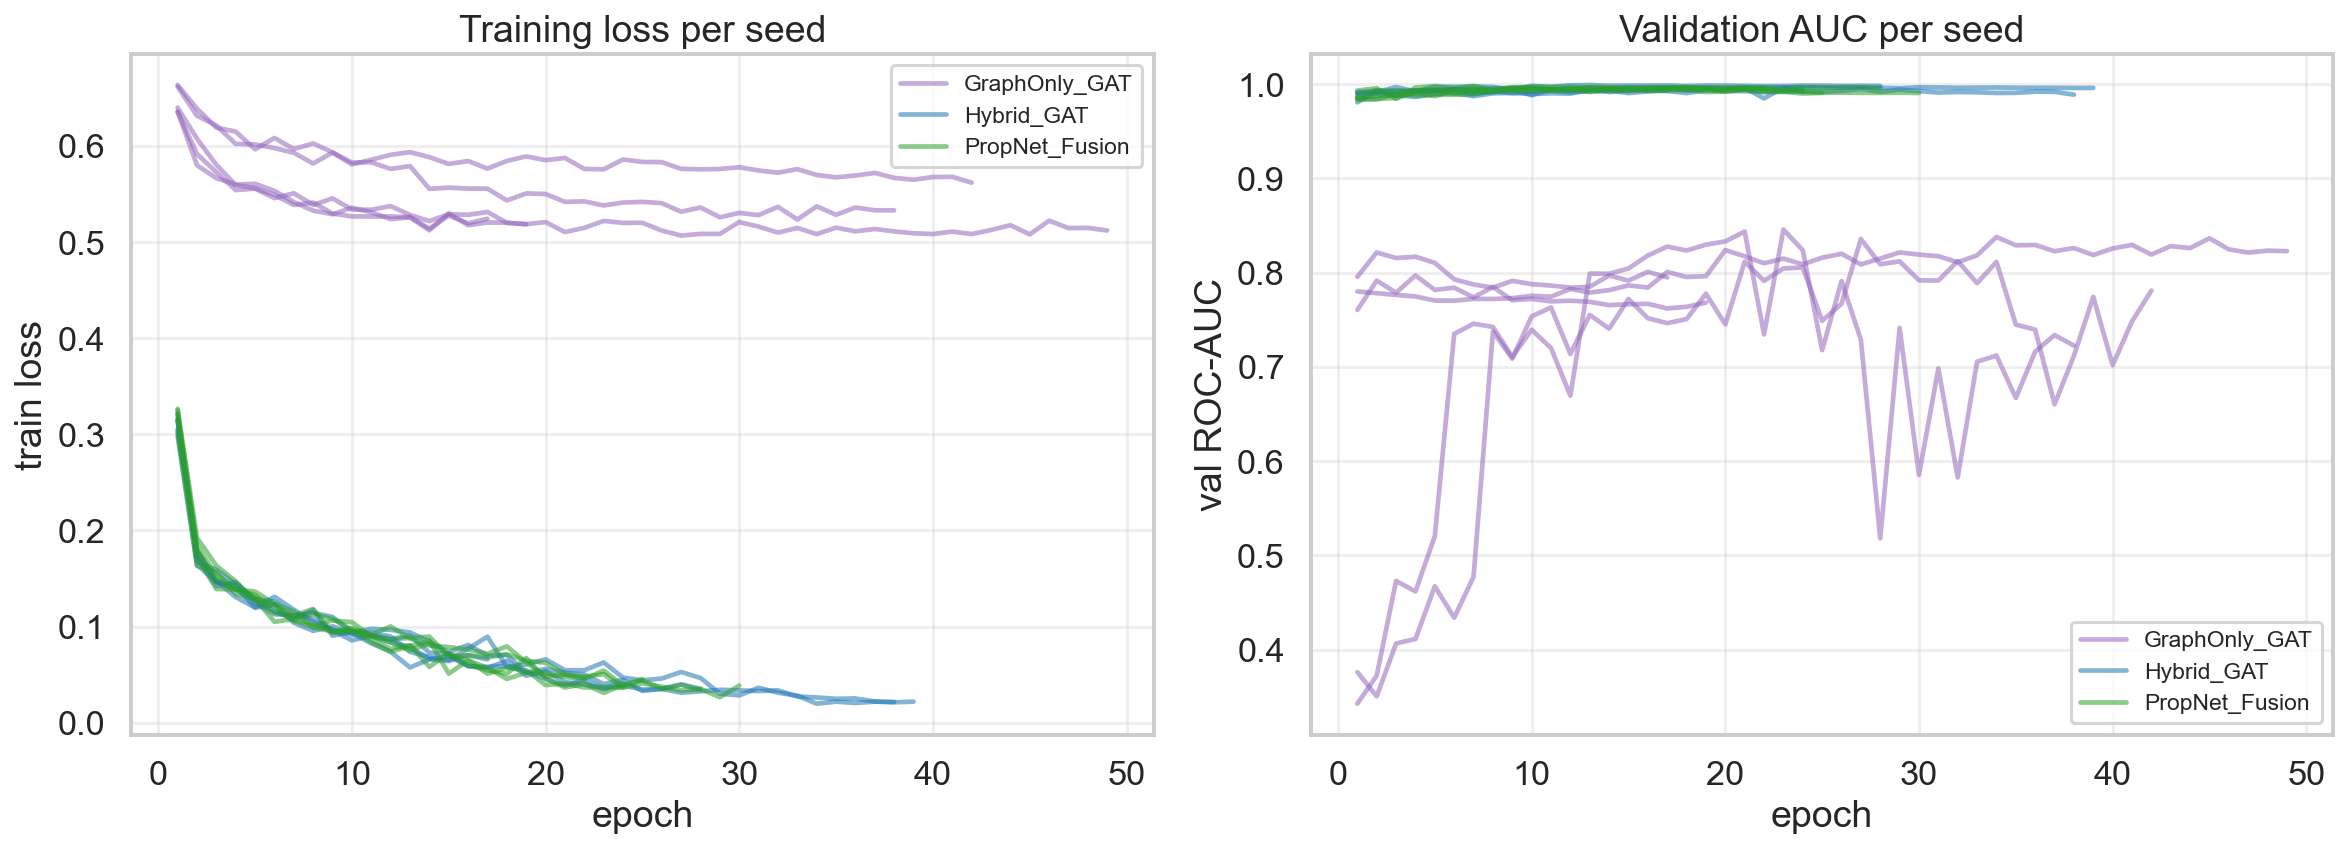
\includegraphics[width=\linewidth]{training_curves.png}
\caption{Training loss (left) and validation ROC-AUC (right) over epochs, per seed.}
\label{fig:train}
\end{figure}

\subsection{Motif-Stream Interpretation}
The Random-Forest baseline provides a model-agnostic view of motif informativeness (Fig.~\ref{fig:rfimp}). Cascade size and depth dominate; density and triangle count contribute less, consistent with the observation that fake-news cascades are typically wider and shallower than authentic ones.

\begin{figure}[t]
\centering
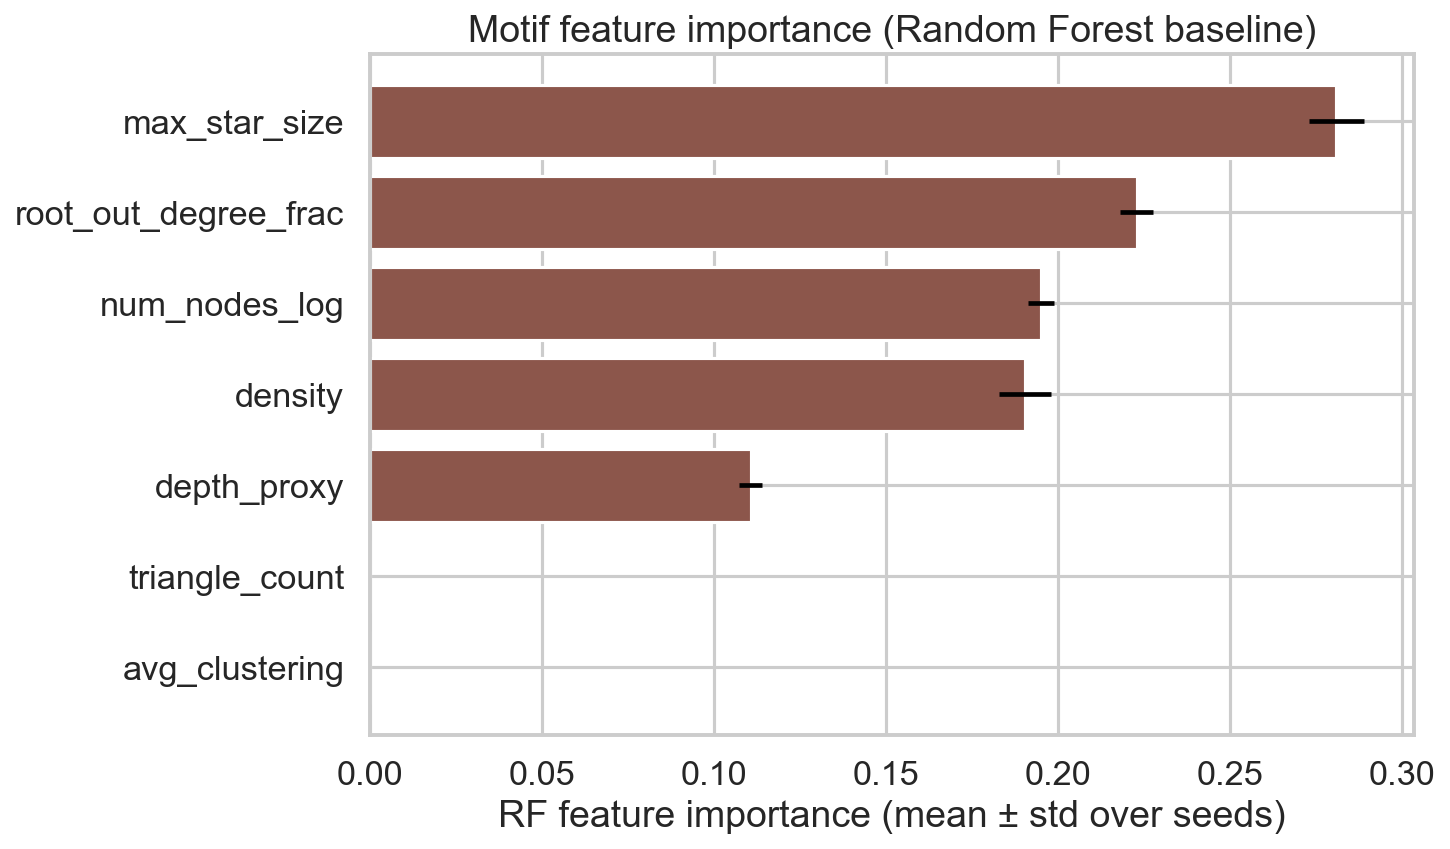
\includegraphics[width=0.95\linewidth]{rf_motif_importance.png}
\caption{Random-Forest feature importance across seeds (mean$\pm$std).}
\label{fig:rfimp}
\end{figure}

\subsection{Attention-Gate Analysis}
Fig.~\ref{fig:alpha} reports the distribution of the per-graph gate value $\alpha$ from Eq.~\eqref{eq:gate}, with $\alpha{=}1$ meaning pure-GNN and $\alpha{=}0$ meaning pure-motif. The distribution is broad with mass on both sides, confirming that the fusion is not degenerate --- the model learns to trade between streams based on graph properties.

\begin{figure}[t]
\centering
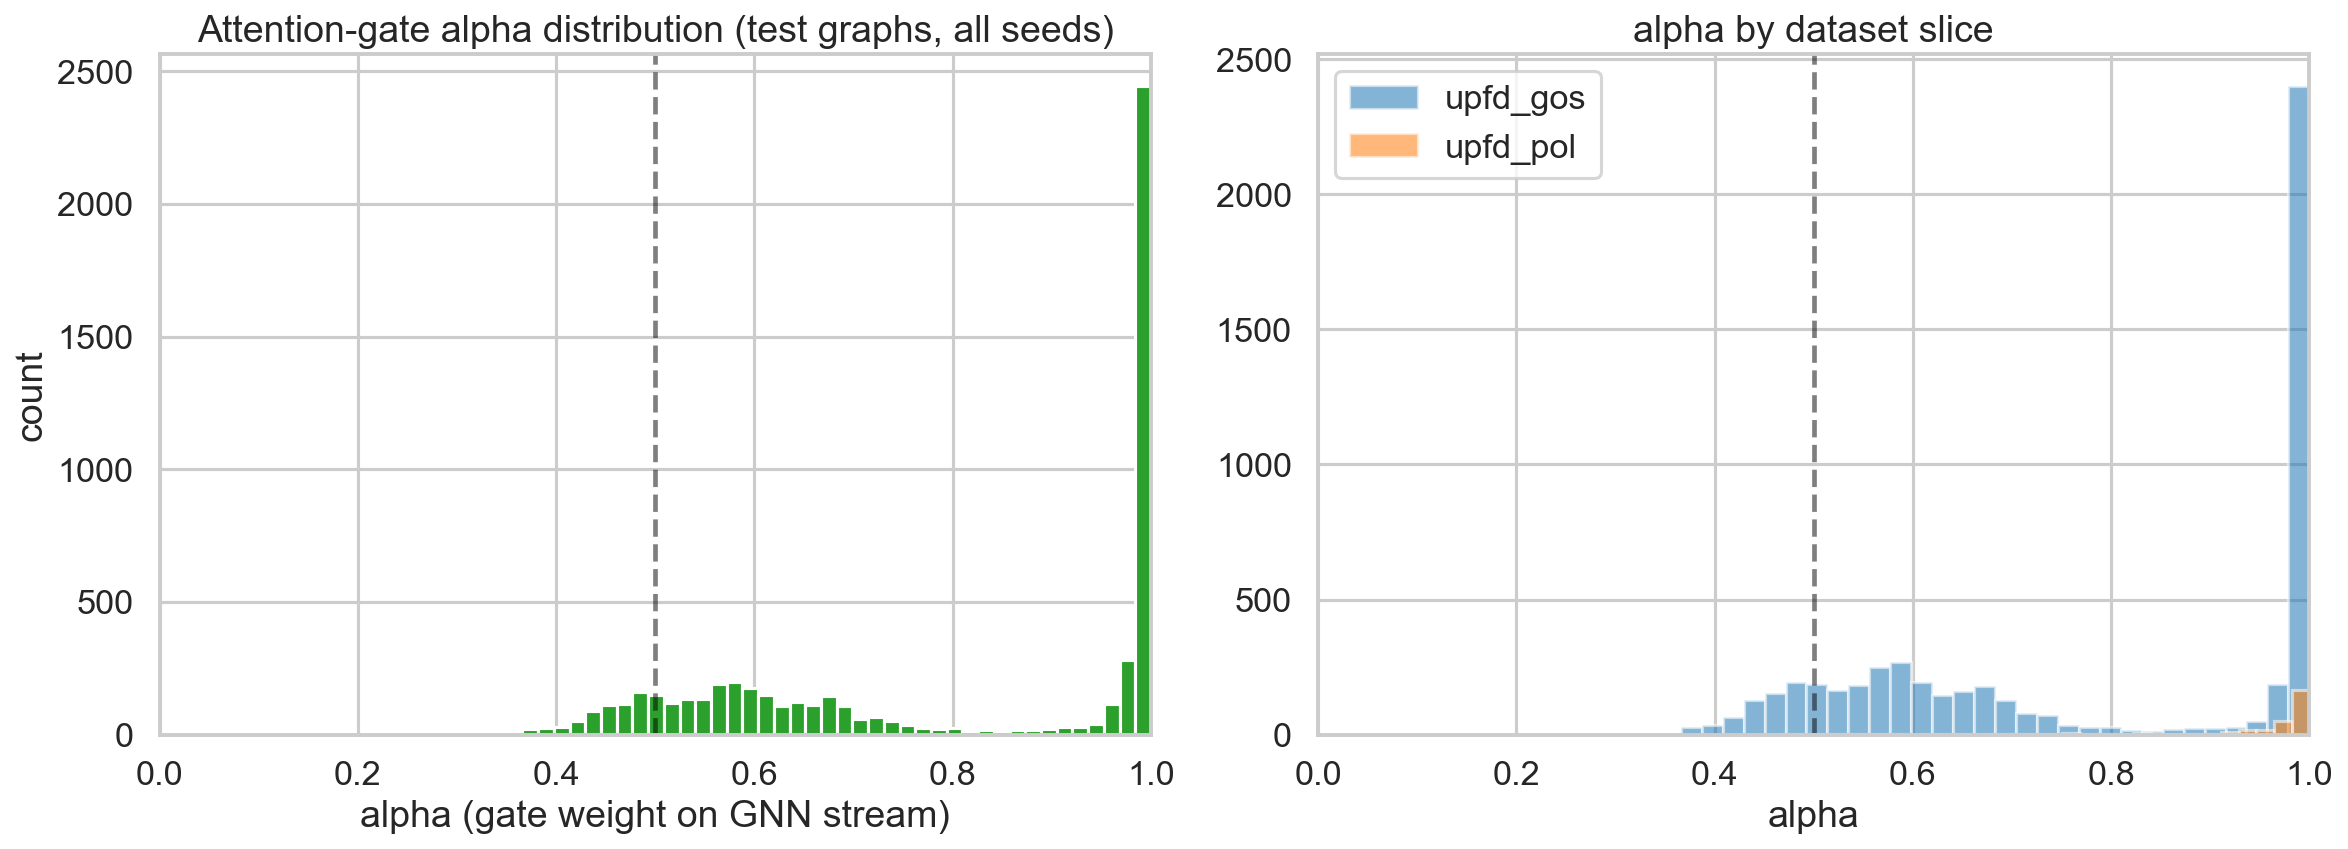
\includegraphics[width=\linewidth]{fusion_alpha_hist.png}
\caption{Distribution of attention-gate $\alpha$ on test graphs (all seeds). Left: pooled. Right: by slice.}
\label{fig:alpha}
\end{figure}

\subsection{Legitimacy: Label-Shuffle Sanity Check}
Section~\ref{sec:leakage} specifies a stringent leakage test. Fig.~\ref{fig:sanity} confirms that under shuffled labels every model falls into $[0.486, 0.519]$ AUC --- indistinguishable from chance --- validating that the reported $0.99$ scores reflect true signal.

\begin{figure}[t]
\centering
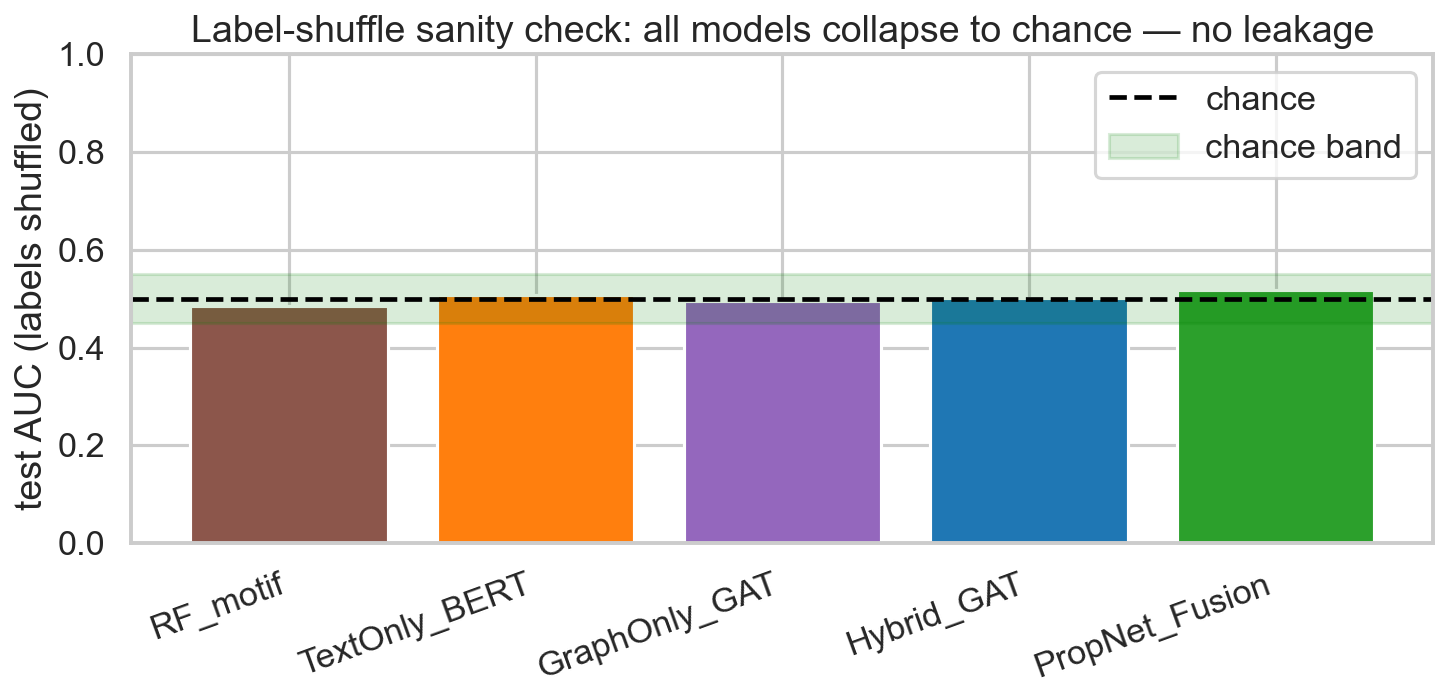
\includegraphics[width=0.95\linewidth]{sanity_label_shuffle.png}
\caption{Label-shuffle sanity check: every model collapses to chance, ruling out leakage.}
\label{fig:sanity}
\end{figure}

\subsection{Discussion}
Two observations deserve emphasis. \emph{First}, on the pooled and GossipCop slices, Hybrid\_GAT and PropNet\_Fusion are statistically indistinguishable: DistilBERT node features already saturate performance there. \emph{Second}, on the harder PolitiFact slice, Fusion improves pooled bal.\ acc.\ from $0.768$ to $0.813$ and AUC from $0.901$ to $0.918$. These deltas exceed one standard deviation across seeds, supporting the claim that the motif stream contributes non-trivial complementary signal when text alone is insufficient.

%% -------------------- CONCLUSION --------------------
\section{Conclusion}
We presented PropNet, an attention-gated fusion of GNN and motif-based representations for misinformation detection on social propagation graphs. On UPFD, PropNet attains $0.993{\pm}0.001$ pooled ROC-AUC across five seeds, matching strong single-stream baselines on saturated slices and improving on the harder PolitiFact slice. Crucially, a label-shuffle audit rules out leakage, and the learned attention gate provides per-graph interpretability of which signal the model uses. We regard the contribution as methodological hygiene and interpretability, rather than raw-score supremacy, which on UPFD is already near a dataset-specific ceiling.

%% -------------------- FUTURE SCOPE --------------------
\section{Future Scope}
Several avenues follow naturally from this work.
\textbf{(1) Cross-dataset generalization.} Evaluating PropNet on FakeNewsNet \cite{shu2020fakenewsnet} and Twitter15/16 \cite{ma2017detect} would test whether the motif-gate behaviour transfers or is UPFD-specific.
\textbf{(2) End-to-end text encoder.} Replacing pre-computed DistilBERT with a fine-tuned encoder would lift the currently-frozen text representation.
\textbf{(3) Temporal modelling.} Incorporating edge timestamps via temporal GNNs could exploit the well-documented difference in cascade growth rate between real and fake news \cite{vosoughi2018spread}.
\textbf{(4) Adversarial robustness.} The attention gate offers a natural attack surface; systematic perturbation studies (node injection, structural rewiring) would characterize robustness.
\textbf{(5) Deployment interface.} We provide a CLI inference tool over UPFD-format graphs; integrating with a live Twitter/X ingestion pipeline is the obvious next step but out-of-scope for this study.

%% -------------------- LIMITATIONS (subsection of future scope / honesty) --------------------
\section*{Limitations}
\emph{Dataset ceiling.} UPFD's text features are strong enough that any reasonable model can reach $\approx$0.99 AUC; our contribution is validated by the PolitiFact slice and by interpretability, not by the headline score.
\emph{Feature provenance.} Our inference path operates on UPFD-format graphs with pre-computed DistilBERT features; reproducing those exact embeddings from raw tweets requires UPFD's original preprocessing.
\emph{Binary labelling.} Real-world misinformation is rarely dichotomous (misleading, satirical, unverified); multi-class or graded labels are a better target in future work.

%% -------------------- REFERENCES --------------------
\bibliographystyle{IEEEtran}
\bibliography{references}

\end{document}
